%  ProjectManagement.tex
%  Document created by seblovett on seblovett-Ubuntu
%  Date created: Thu 17 Apr 2014 15:26:37 BST
%  <+Last Edited: Mon 12 May 2014 16:03:00 BST by seblovett on seblovett-Ubuntu +>

\chapter{Project Management}\label{ch:pm}
%\incomplete{Project Management}


Groups members are referred to by initials in this Chapter as follows:
\begin{enumerate}
\item HL - Henry Lovett (hl13g10)
\item MW - Martin Wearn (mw20g10)
\item AJR - Ashley Robinson (ajr2g10)
\item ARR - Anusha Reddy (arr1g13)
\end{enumerate}

\section{Group formation}

The group initially contained five students. 
At the start of the project, two of the original students left the group: one joined another team, and one dropped the module.
This left the group with three members - AJR, MW and HL. 
Discussions were then undertaken as to if the group wanted / needed a fourth member. 
As the group could not come to a unanimous decision, one for a fourth member, one against and one who was happy either way, Iain's advice for having a fourth member was taken. 

The original member of the group did not wish to rejoin the group.
Instead, a colleague of the original member was offered to join.
%This formed the group members. 

In the first discussions with the group, HL was appointed as group leader. 

\section{Meetings}

The group held two meetings per week at scheduled times: Monday afternoons at 15:00 and Thursday afternoons at the end of the lab.
%A meeting was always held towards the end of the Thursday lab session.
All meetings were chaired by HL.

Agendas for Monday meetings were sent out by HL, usually 24 hours beforehand. 
The Monday meeting was there to discuss any work done since Thursday or outstanding issues. 
The other task for the Monday meeting was to confirm the milestones for the week.
This ensured that all group members were aware of who was responsible for what that week to avoid confusion that could potentially cause a delay in a hand-in.
Ongoing tasks were discussed at these meetings also.
Work for the lab on Thursday was allocated so members were able to commence work without hindrance.

The meeting at the end of the Thursday lab was to discuss the progress made that day. 
As this was the main working time, smaller aspects were discussed during the day between individual members.
The meeting at the end of the lab allowed everyone to know any design changes or issues encountered and the problems discussed.
Work for the time outside of the lab was then allocated at this point.


\section{Skills Assessment}

A small skills audit was done in the first meeting. 
The results of this are seen in Table~\ref{tab:pm:skills}.
It was apparent early on that ARR was not comfortable with a lot of the skills required.
Realising this early in the project allowed the work to be allocated optimally throughout the group members, particularly ensuring ARR was given realistic objectives and adequate help where required.

\begin{table}[h]
\centering
\caption{Skills Audit for Team R4. A 5 means very competent, 1 is not competent.}
\label{tab:pm:skills}
\begin{tabular}{l*{4}{p{1cm}}}\hline
Task 			& HL & MW & AJR & ARR \\ \hline
Verilog 		& 4  & 4  & 4   & 2   \\
Magic Layout		& 4  & 4  & 3   & 4   \\
Assembly Language	& 3  & 3  & 3   & 1   \\
Processor Design	& 4  & 4  & 4   & 1   \\ 
Git			& 4  & 3  & 4   & 1   \\ \hline
\end{tabular}
\end{table}


\section{Work Breakdown}

The skills audit provided the basis for the initial work allocations.
Preferences were given and the group was roughly broken into two sections: HL and AJR were to pursue the SystemVerilog development, MW and ARR would do the Magic layout.
Although the work was distributed this way, it was by no means a comprehensive divide.
ARR and MW were to also write SystemVerilog testbenches, and HL and AJR would be responsible for the synthesis and layout of the control unit.
The initial breakdown was done to give the team a starting point.

%The milestone responsibilities were also allocated, loosely based on the skills audit.


\section{Git}
%Git was used for revision control and branching (interrupt development)

HL, MW and AJR all had worked together previously, therefore the use of Git revision control was decided before the group was formed. 
When ARR joined the group, our file control was discussed, and alternative options were discussed. 
One idea from ARR was to use DropBox. 
This was a simple to use system, but would cause issues when multiple people worked on the same files. 
There was also no log of changes and broken files could have accidentally been integrated. 
The full recursive revision control with Git helped as if and when a file was committed that didn't work, it could be reverted to the previous version.
Change logs are also used with Git, allowing to see which files have changed, by who and why. 


The advantage to using Git was that the work could be branched.
This was exceptionally useful as the group was looking to implement interrupts.
The interrupt work could be done concurrently, but separately, to the normal work flow. 
If the group hadn't achieved the milestones for the interrupt development, no time would have been needed removing it.
At the point of success with interrupts, the work done was easily merged into the master branch. 

All group members agreed on the use of Git. 
HL and MW both spent time with ARR to help her understand the basics to be able to use Git.


\section{Github}
%Issue Tracking and task allocation using GitHub
Github is an online resource for hosting Git repositories. 
As well as the hosting, Github provides an issue tracking facility.
Issues were opened for items of work to be done, or for bugs found in the design.
The issue webpages provided a comment thread for the group members for discussion.

Issue tracking meant it was easy to keep an eye on what tasks were on going, complete or if it needed more time and resources to complete on time.
Issues can be allocated to group members, so the same task is not completed by multiple people. 
Github was extremely useful for this tracking and provided a common communication network for the group. 

\subsection{Git Additions by Group Member}

Github has the ability to extract statistics of the repository. 
This includes the commits, additions and deletions over time by each user (excluding merges). 
The number of commits is not an accurate method of measuring activity as different people have different commit habits.
For example, one member may commit a lot, but make little changes in each commit, whereas someone else may make a lot of changes, test and then commit.
Deletions are also included in the statistics, but are not a reliable measure as HL was responsible for keeping the repo clean and removing the temporary or unused files. 

However, the total additions is a more accurate measure. 
Magic files can be included in this measure as these are plain text files.
Report writing was done using \LaTeX, which in essence, is code and therefore the additions measure applies here too.

Due to ARR being introduced to Git, it would be expected that in the initial phase of the project, her commit count would be low, resulting in low additions also. 
Ideally, this would then increase to a reasonable level during the project. 
Some commits were done on behalf of ARR by HL in the early stages also, but this was not common.

Figure~\ref{fig:additions} shows the addition history in the repository. 
It is clear to see that HL employs a commit little and often style, where as MW and AJR commit more in less commits. 
The initial peak with AJR was the addition of an emulator he found.
If this is not taken into account, the total additions of HL, AJR and MW are approximately equal.  
It was expected that the additions of ARR would be lower than other members due to the learning curve needed for Git.
However, it is clear to see the 6,225 additions from ARR is significantly less than the rest of the group.

\begin{figure}
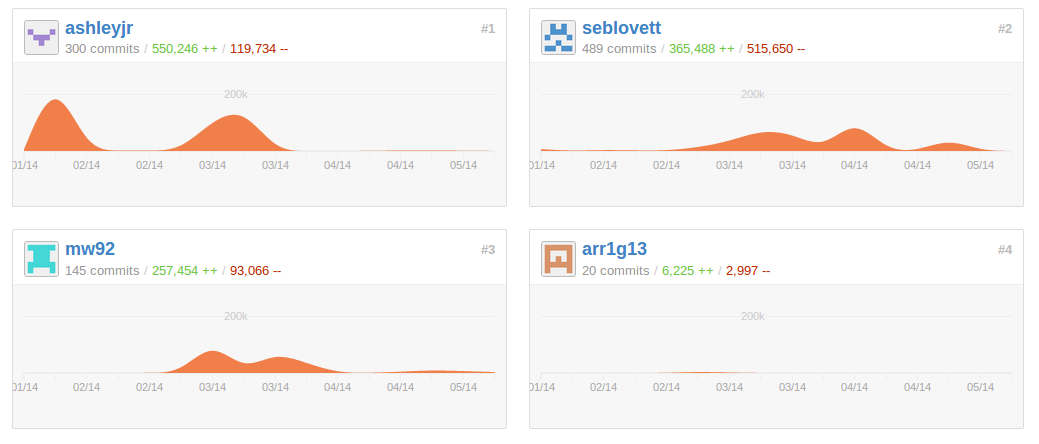
\includegraphics[width=\textwidth]{Figures/gitadditions.png}
\caption{Graph from Github showing the additions over time for each user. Additions are measured in lines in a file and shown in green. Deletions are shown in red. (seblovett = HL; ashleyjr = AJR; mw92 = MW; arr1g13 = ARR)}
\label{fig:additions}
\end{figure}


\section{Reflections}

This section contains individual reflections from group members. 
These are written to give everyone a chance to discuss their view of the group operation. 
ARR's reflection is not included. 
She was advised to include her own reflections in her individual report and given the same suggestions as to what it should include.

\subsection{HL}

\subsection{MW}

\subsection{AJR}

%\subsection{ARR}

